\chapter{Approach\label{chap:Approach}}

The subject of this thesis is the advancement of compositional techniques for circuit synthesis. We start by discusssing our contribution to the compositional circuit synthesis based on STGs and present the resynthesis technique. Next we introduce the parametrised graphs formalism naturally supporting compositional reasoning. 


\section{Overview}
Handshake circuits~\cite{van2004handshake} are widely applied in the design and synthesis of real-life hardware.
One prominent problem is obtaining an efficient implementation from a \emph{structural} compositional specification.
Syntax-based synthesis tools such as Balsa~\cite{balsa} are unable to take into account the compositional
behaviour of STGs corresponding to handshake circuit components. To address this issue we propose 
a technique that selectively composes STGs of related components to obtain a smaller and more performant
circuit without suffering state space explosion commonly associated with Petri net based techniques~\cite{Valmari}.
This transformation, which we refer to as \emph{resynthesis}~\cite{ukaf_balsa_resynthesis}, is accomplished in three stages. First, we apply a heuristic to identify the most promising candidates for STG-level composition. Second, we perform a parallel composition of the selected component STGs and as a result obtain a new handshake circuit with custom components, functionally equivalent to a combination of elementary components. Finally, a gate-level implementation is obtained from the new handshake circuit via a component-wise synthesis of STGs.

Unfortunately, the standard definition of parallel composition almost always yields a `messy' Petri net, with many implicit places, causing performance deterioration in techniques that are based on structural methods such as the resynthesis approach. To counter this, we propose an improved algorithm for computing the parallel composition. The algorithm generally produces nets with fewer implicit places that are better suited for subsequent application of structural methods~\cite{improved_par_comp}.

In addition to purely structural composition of STGs, it is also beneficial to consider a mixture of 
structural and behavioural composition. Conditional Partial Order Graphs (CPOG)~\cite{2009_mokhov_phd} is a graph-based notation supporting compact
representation and efficient manipulation of both structural and behavioural composition styles. As one example, when developing complex circuit, it is
often necessary to consider several operational modes of a circuit. 
For this, one needs methodologies and tools to exploit similarities between
the individual modes and hence lift the level of discourse to behaviour families.
This necessitates that behaviours are managed in a compositional
way: the specification of the system must be composed from specifications
of its blocks. Furthermore, since the approach is intended to be a part of a safety critical toolchain, it is essential that such a  specification is amenable to mechanised reasoning and transformation.

In Chapter~\ref{chap:PGAlgebra} we propose an extension of the CPOG formalism, called Parameterised Graph (PG).
PGs deal with general graphs rather than just partial orders. We introduce an algebra of Parameterised Graphs by specifying the
equivalence relation via a set of axioms, which we prove to be sound,
minimal and complete~\cite{pg_algebra}. This result allows one to manipulate a PG model
as an algebraic expression applying the bi-directional rewrite rules of this algebra. This is  in contrast to the CPOG formalism that does not offer a unifying algebraic structure. We demonstrate
the usefulness of the developed formalism with two case studies coming
from the area of microelectronics design.

The CPOG formalism can be applied to merge several distinct behaviours
into a single compact CPOG~\cite{2009_mokhov_phd}. As one example, this has been previously used to
synthesise control logic for instruction decoding. In this thesis (Chapter~\ref{chap:PGEncoding}) 
we improve upon this work by offering a powerful technique to automatically discover an optimal encoding and
synthesise a matching optimal decoding circuit. From the outset, we consider a larger set of potential solutions
which enables us to formulate the global optimality criterion. We use an automated satisfiability solving 
techniques to find an optimal solution~\cite{cpog_encoding}.


\section{Balsa Resynthesis\label{sec:Balsa-Introduction}}

The main obstacle for the wider acceptance of asynchronous systems is the inherent complexity of their design. Several solutions are
accepted by the industry to help to simplify the design process through abstraction
of predesigned asynchronous circuit parts as standardised high level
components. A designer is able to use these components as ``building
blocks'', and then obtain the final gate-level design through an
automated mapping process. Some of the well-known asynchronous
design automation packages, such as Tangram~\cite{951597}, and Balsa~\cite{balsa},
define a high-level programming language that is used to describe
systems. The language constructs are then directly translated into
a network of \emph{handshake components}-- blocks with predefined
functionality that use \emph{handshakes} to interface with other components,
which are in turn mapped into a gate netlist~~\cite{van2004handshake}.

Although this method greatly enhances the designer's productivity,
it has several important drawbacks. Of these, the control-path overhead
is the most decisive. The controllers obtained by syntax-directed
mapping are usually far from optimal because the predesigned components
are required to implement their declared protocols fully and correctly
in order to be reusable in all possible circuit configurations. However,
it is often the case that a significant part of their functionality
becomes redundant due to the peculiarities of the specific configuration,
e.g. in many cases full handshaking between the components can be
avoided.

This redundancy may be eliminated by replacing a manually designed
gate-level implementation of the high level components with an equivalent
STG~(signal transition graph) specification~\cite{Yakovlev_1998_cs}.
The STGs of individual components are then composed together to form a
 STG representation of the whole system STG~\cite{785214} and is optimised with \noun{petrify~}\cite{cortadella_petrify}.
An optimal gate-level implementation is then automatically produced
from the STG using tools such as \noun{petrify}~\cite{cortadella_petrify},
\noun{SIS}~\cite{Sentovich:M92/41} and \noun{MPSat}~\cite{Khomenko_2004_MPSAT}.
Automatic synthesis becomes problematic when the size of a STG becomes
large: modern synthesis tools can handle STGs of no more than 100
signals. The impact of this problem can be lessened by including STG decomposition tools~\cite{DesiJ} into the workflow. They break a large, optimised STG down into several smaller STGs that are synthesisable
in reasonable time. Alternatively, the decomposition step is carried
out at the level of handshake circuits, dividing a circuit into several
smaller blocks of components.

\section{Petri Nets}\label{sec_pn_basic}

% ***************** Petri Net Basics ********************
A \emph{Petri net} is a 4-tuple $N=(P,T,W,M_N)$ where
$P$ is a finite set of \emph{places} and $T$ is a finite set of \emph{transitions}
with $P \cap T=\emptyset$,
$W: P\times T \cup T \times P \rightarrow \nat_0$ is the \emph{weight function,} and
$M_N$ is the \emph{initial marking}, where a \emph{marking} is a multiset of places,
\ie a function $P\rar\nat_0$ which assigns a number of \emph{tokens} to each place.
A Petri net can be considered as a bipartite graph with weighted arcs between places and transitions.
If necessary, we write $P_N$ etc.\ for the components of $N$ or $P'$ ($P_i$) etc.\ for the net $N'$ ($N_i$) etc.


% ***************** Preset, Postset ********************

The \emph{preset} of a place or transition $x$ is denoted as $\pre x$ and defined by
$\pre x\DEF\{y\in P\cup T\ |\  W(y,x)>0\}$,
the \emph{postset} of $x$ is denoted as $\post x$ and defined by
$\post x\DEF\{y\in P\cup T\ |\ W(x,y)>0\}$.
These notions are extended to sets as usual.
We say that there is an \emph{arc}
from each $y\in \pre x$ to~$x$.




% ***************** Enabledness, Reachable States ********************

A transition $t$ is \emph{enabled under a marking M}
if $\forall p\in \pre t:M(p)\geq W(p, t)$, which is denoted by $M\tfrs t$.
An enabled transition $t$ can \emph{fire} yielding a new marking $M'$,
written as $M\tfrs t M'$,
where $M'(p)=M(p)-W(p, t) + W(t,p)$, for all $p\in P$.
A transition sequence $\sigma=t_1\ldots t_n$ is \emph{enabled under a marking $M$} (yielding $M'$)
if $M\tfrs{t_1}M_1\tfrs{t_2}\ldots M_{n-1}\tfrs {t_n} M_n=M'$, and we
write $M\tfrs \sigma$, $M\tfrs \sigma M'$ resp.; $\sigma$ is called \emph{execution of $N$} if $M_N\tfrs \sigma$.
  The empty transition sequence $\lambda$ is  enabled under every marking.
$M$ is called \emph{reachable} if a transition sequence $\sigma$ with
$M_N\tfrs \sigma M$ exists.

$N$ is called \emph{bounded} if, for every reachable marking $M$ and every place $p$, $M(p)\leq k$ for some constant $k\in \nat$; if $k=1$, $N$ is called \emph{safe}. $N$ is bounded if and only if the set $\tfrs {M_N}$ of reachable markings is finite. In this thesis, we are mostly concerned with bounded Petri nets.

A place $p$ is \emph{implicit} if it can be deleted from the net
without changing the set of executions, and so an implicit place can be removed from the net without affecting its behaviour.\footnote{Note that an implicit place can cease to be implicit if another implicit place is removed first.}
Unfortunately, detecting
implicit places is expensive: the problem is \PSPACE-complete for safe and \EXPSPACE-complete for general Petri nets. A place $p$ is \emph{duplicate} if there is another place $p'$ with the same pre- and postsets whose initial marking does not exceed that of $p$. Duplicate places are implicit, and are cheap to detect.

\smallskip

An \emph{STG} is a tuple $N=(P,T,W,M_N,\I,\Ot,\ell)$ where
$(P,T,W,M_N)$ is a Petri net and $\I$ and $\Ot$  are disjoint
sets of \emph{input} and  \emph{output signals}. For
$\Sig=\I\cup\Ot$ being the set of all signals,
$\ell:T\rightarrow\Sig\times\{+,-\}\cup \{\lambda\}$ is the
\emph{labelling} function. $\Sig\times\{+,-\}$ or short
$\Sig\upd$ is the set of \emph{signal transitions}; its
elements are denoted  as $s^+$, $s^-$  resp.\ instead of
$(s,+)$, $(s,-)$ resp. A plus sign denotes that a signal value
changes from \emph{logical low} (written as 0) to \emph{logical
high} (written as 1), and a minus sign denotes the opposite
direction. We write $s\upd$ if it is not important or unknown
which direction takes place.

An STG can contain transitions labelled with $\lambda$, called
\emph{dummy} transitions, which do not correspond to any signal
change. \emph{Hiding a signal $s$} means to change the label of
all transitions labelled with $s\upd$ to $\lambda$. (The idea
of re-synthesis approach is to hide the signals used for
communication between components, which results in an STG with
fewer signals that often has a simpler implementation as a
circuit.) The labelling of an STG is called \emph{injective} if
for each pair of distinct non-dummy transitions $t$ and $t'$,
$\ell(t)\neq\ell(t')$.

\smallskip

Examples of STGs are shown in Figs.~\ref{fi-motivating-example1} and~\ref{fi-motivating-example2}.
Places are drawn as circles containing a number of tokens corresponding to the initial marking.
Unmarked places which have only one transition in their presets and postsets are
not drawn if the corresponding arcs have the weight~1; they are implicitly
given by an arc between these two transitions (and if such a place contains tokens, they are drawn on the arc itself). Transitions are drawn simply as their labels,
and the weight function is drawn as directed arcs $(x,y)$ whenever $W(x,y)\neq 0$ (and
labelled with $W(x,y)$ if $W(x,y)>1$).


\smallskip

% ********************** labels ***************************

We lift the notion of enabledness to transition labels: we write
$M\ifrs {\ell(t)}  M'$ if $M\tfrs t  M'$. This is extended to sequences
as usual -- deleting $\lambda$-labels automatically since $\lambda$
is the empty word; \ie $M\ifrs{s\upd}M'$ means that a sequence of
transitions fires, where one of them is labelled $s\upd$ while the
others (if any) are $\lambda$-labelled. A sequence
$\nu\in(\Sig\upd)^*$ is called a \emph{trace of a marking} $M$ if
$M\ifrs \nu$, and a \emph{trace} of $N$ if $M=M_N$. The \emph{language $L(N)$
of $N$} is the set of all traces of $N$.

\smallskip

The \emph{reachability graph} $\RG(N)$ of an STG $N$ is an arc-labelled
directed graph on the reachable markings of $N$ with $M_N$ as the root;
there is an arc from $M$ to $M'$ labelled $\ell(t)$ whenever
$M\tfrs {t} M'$. For bounded Petri nets and STGs, $\RG(N)$ can be seen as a finite automaton
(where all states are accepting), and $L(N)$ is the language of this
automaton.
Observe that automata with accepting states only can be
regarded as STGs (with the states as places, the initial state being the
only marked place, etc.); hence, all definitions for STGs also
apply to automata.

$N$ is \emph{deterministic} if $\RG(N)$
is a deterministic automaton: it contains no $\lambda$-labelled transitions
and there are no \emph{dynamic auto-conflicts,} \ie for each reachable marking $M$ and each signal transition $s\upd$
there is at most one $M'$ with $M \ifrs {s\upd} M'$. (Note that a deterministic STG
can have choices between different outputs, \eg an STG modelling
the standard arbiter is deterministic).

An STG with a set of all markings $S_2$ is said to \emph{simulate} another STG with 
a set of all markings $S_1$ iff there exist an 
$R \subset S_1 \times S_2$ such that $(M_{N 1},M_{N 2}) \in R$ and for any pair of markings 
$(M_1, M_2) \in R$, a label $l$ and a marking $M_1'$, $M_1\ifrs {l}  M_1'$ implies 
$M_2 \ifrs {l} M_2'$ for some $M_2'$. We call $R$ the witness of simulation. Now we can say that STGs $N_1$ and $N_2$ are \emph{bisimilar} iff $N_2$ simulates $N_1$ with witness $R$ and $N_2$ simulates $N_1$ with witness $R^{-1}$.

For deterministic STGs, language equivalence and bisimulation coincide, and the language can be taken as the semantics of such a specification. Unfortunately, the class of deterministic STGs is too restrictive in practice~\cite{KSV-08}, \eg:
\begin{itemize}
  \item using dummy transitions is often convenient in manual design;
  \item modelling OR-causality~\cite{ykklp96} as a safe STG requires non-determinism;
  \item hiding internal communication (and thus introducing dummy transitions) is a crucial step in re-synthesis.
\end{itemize}
Hence, one has to deal with non-deterministic STGs as well.

One might think that if $\RG(N)$ is non-deterministic, it can be \emph{determinised} (using well-known auto\-ma\-ta-the\-o\-re\-tic methods), \ie turned  into a language-equivalent deterministic
automaton with accepting states only; in particular, the resulting automaton will have no $\lambda$-arcs. Unfortunately, this is a bad idea, as shown in~\cite{KSV-08}, where the semantics of non-deterministic STGs was developed. It is based on the concept of \emph{output-determinacy,} which is a relaxation of determinism: An STG $N$ is \emph{output-determinate (OD)} if $M_N \ifrs {\nu}
M_1$ and $M_N \ifrs {\nu} M_2$ implies for every $x\in \Ot_N$ that
$M_1 \ifrs {x\upd}$ iff $M_2 \ifrs {x\upd}$.
It turns out that OD STGs are exactly the STGs which
have correct implementations according to the implementation relation introduced in~\cite{KSV-08}.
Hence, non-OD STGs are ill-formed, and in particular cannot be correctly implemented as
circuits. This shows that in general, \emph{the language is not a satisfactory semantics of
non-deterministic STGs;} in particular, \emph{synthesising the determinised reachability graph of a non-OD STG
will either fail or result in an incorrect circuit.} On the other hand, for the class of OD STGs~\cite{KSV-08} shows that their language
is an adequate semantics, and
implementation relation can be formulated purely in terms of the language.
An important property of OD STGs is that in them the enabledness of an output signal is a function of the trace, \ie given a trace $\nu$, the set of outputs by which $\nu$ can be extended is uniquely determined, even though there could be multiple executions corresponding to $\nu$.


\smallskip

In the following definition
of {\em parallel composition}~$\parallel$, see \eg~\cite{vowo02lncs}, we will have to
consider the distinction between input and output signals.
The idea of parallel composition is that the
composed systems run in parallel and synchronise on common actions
-- corresponding to circuits that are connected on the
wires corresponding to the signals.
Since a system controls its outputs, we cannot allow a signal to
be an output of more than one component; input signals, on the other
hand, can be shared.
An output signal of a component may be an input of
other components, and in any case it is an output of the composition.

The parallel composition of STGs $N_1$ and $N_2$ is defined if
$\Ot_1 \cap \Ot_2 = \emptyset$. If we drop this requirement, the
definition gives the {\em synchronous product} $N_1\times N_2$,
which is often useful. The place set of the composition is
the disjoint union of the place sets of the components; therefore,
we can consider markings of the composition (regarded as multisets)
as the disjoint union of markings of the components,
and we will also write such a marking $M_1 \dot{\cup} M_2$
of the composition as $(M_1, M_2)$. To define the transitions,  let
$A=(\I_1 \cup \Ot_1) \cap (\I_2 \cup \Ot_2)$ be the set of
common signals.
If \eg $s$ is an output of $N_1$ and an input of $N_2$,
then firing of $s\upd$ in $N_1$ is `seen' by
$N_2$, \ie it must be accompanied by firing of $s\upd$
in $N_2$. Since we do not know a priori which $s\upd$-labelled
transition of $N_2$ will fire together with some $s\upd$-labelled
transition of $N_1$, we have to allow for each possible
pairing.
Thus, the {\em parallel composition} $N = N_1 \parallel N_2$
is obtained from the disjoint union of $N_1$ and $N_2$ by
fusing
each $s\upd$-labelled transition $t_1$ of $N_1$
with each $s\upd$-labelled transition $t_2$ from $N_2$ if $s \in A$.
Such transitions are pairs and the firing $(M_1, M_2)\tfrs{(t_1,t_2) }(M_1', M_2')$ of $N$
corresponds to the firings $M_i\tfrs{t_i}M_i'$ in $N_i$, $i=1,2$; for an example
of a parallel composition, see Fig.~\ref{fig_parcom}.
More generally, we have $(M_1, M_2) \ifrs{\nu} (M_1', M_2')$ iff
$M_i \ifrs{\nu|_{N_i}} M_i'$ for  $i\in\{1,2\}$, where
$\nu|_{N_i}$ denotes the projection of the trace $\nu$ onto the signals of the STG ${N_i}$.
Hence, all reachable markings of $N$ have the form $(M_1, M_2)$,
where $M_i$ is a reachable marking of $N_i$, $i=1,2$.

Obviously, one can extend the notion of the parallel
composition to a finite family (or collection) $(C_i)_{i\in I}$ of
STGs as $\parallel_{i\in I} C_i$,
provided that no signal is an output signal of more than one of the
$C_i$. We will also denote the markings of such a composition
by $(M_1, \ldots,M_n)$ if $M_i$ is a marking of $C_i$ for
$i\in I=\{1,...,n\}$.
As above, $(M_1, M_2, \ldots, M_n) \ifrs{\nu} (M_1', M_2', \ldots, M_n')$ iff
$M_i \ifrs{\nu|_{C_i}} M_i'$ for all $i\in\{1,\ldots,n\}$.
It is easy to see that $C$ is deterministic if all $C_i$ are. However, this is not true for a composition of OD STGs, as the result, in general, can be non-OD in such a case.

A composition can also be ill-defined due to \emph{computation interference,} see \eg~\cite{eber92}.
Let $C\DEF\parallel_{i\in I}C_{i}$ be a composition of STGs. It is
\emph{free from computation interference (FCI)} if for every trace $\nu$ of $C$
the following holds: if $\nu|_{C_{j}}x^{\pm}$ is a trace of $C_{j}$
for some output $x$ of $C_{j}$, then $\nu|_{C}x^{\pm}$ is a trace
of $C$.

\begin{figure*}[t]
    \centering
    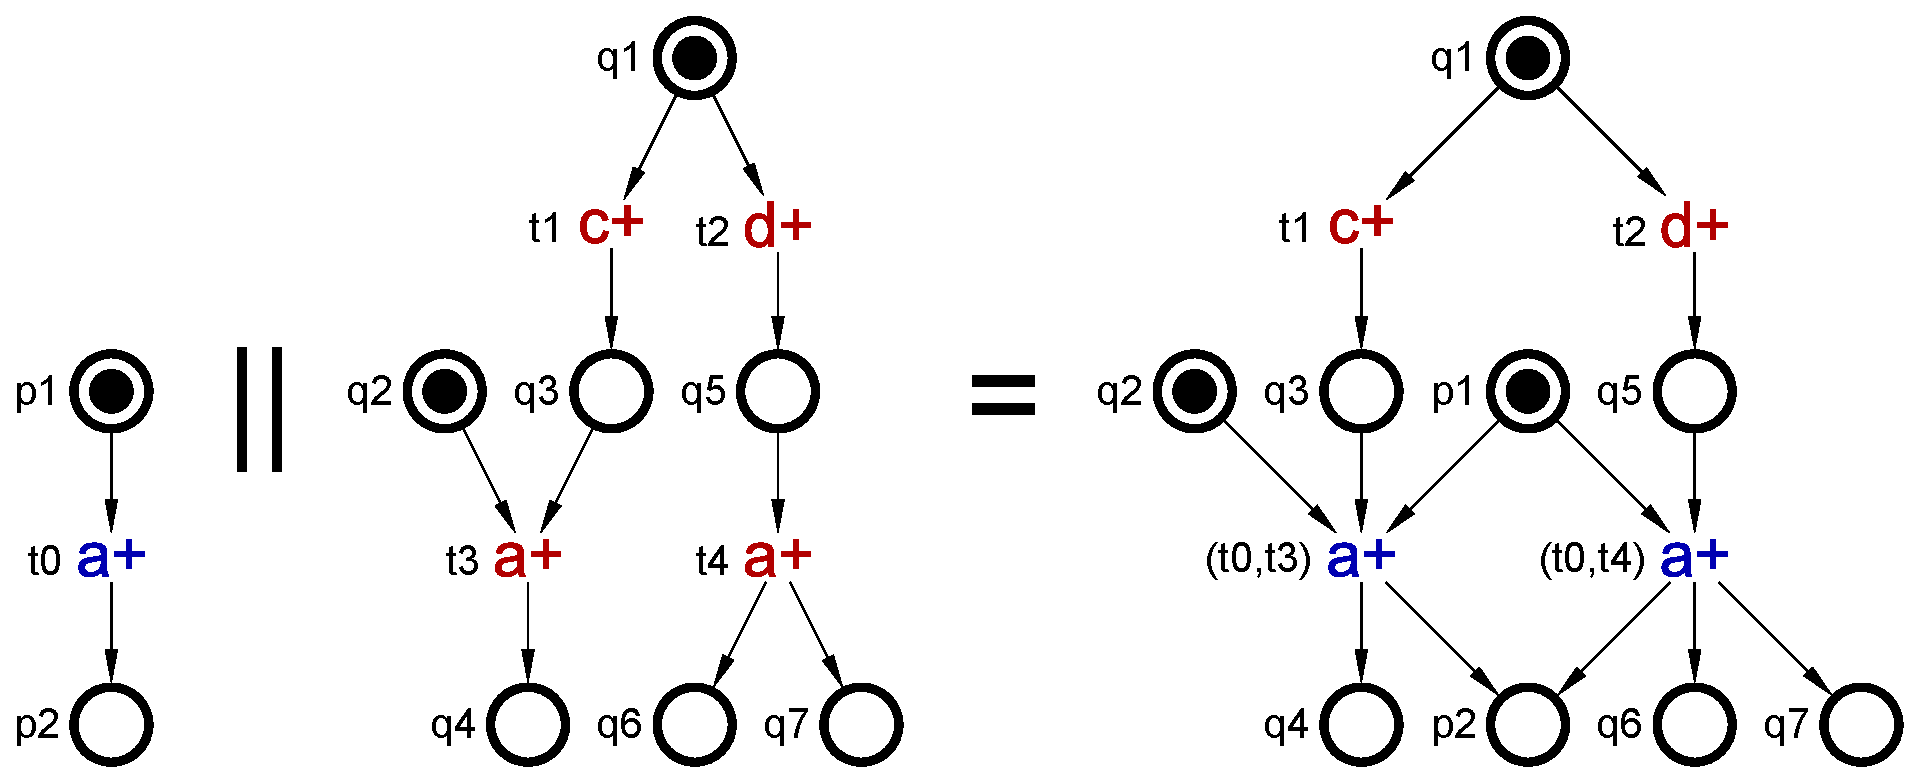
\includegraphics[scale=0.4]{EXPERIMENTS/stg/pcomp_example}
    \caption{\label{fig_parcom}
        Parallel composition example. In the net fragment on the left hand side,
        signal $a$ is an output, and in the fragment in the middle it is an input.
        Hence, in their parallel composition (right) it is an output.
        In this example, there is \emph{computation interference}: the left component activates $a\up$ but the middle one is not ready to receive it.}
\end{figure*}

\smallskip


\begin{figure*}[!tb]
    \centering
    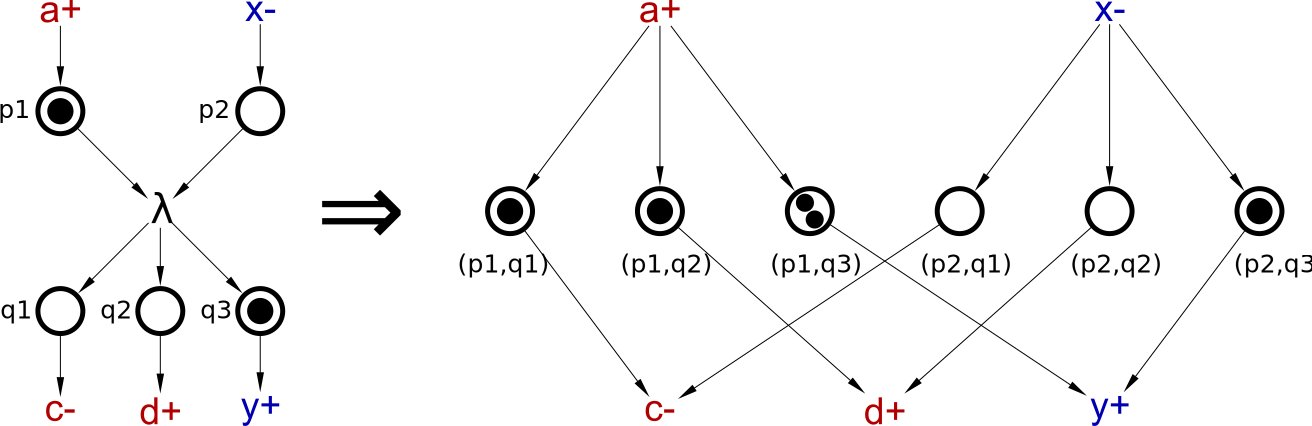
\includegraphics[scale=0.4]{EXPERIMENTS/stg/transition_contraction}
    \caption{\label{fig3.1}
        An example of a transition contraction.
    }
\end{figure*}


\emph{Transition contraction}~\cite{vowo02lncs} is an important operation in circuit re-synthesis. It removes a dummy transition from an STG and
combines each place of its preset with each place of its postset to `simulate' the
firing of the deleted transition, see Fig.~\ref{fig3.1}. Unfortunately, transition contractions are sometimes undefined (\eg in case the transition has a self-loop, \ie some place occurs in both its preset and postset); moreover, even when a contraction is defined, it might change the semantics of the STG.
Hence,~\cite{vowo02lncs} uses the notion of \emph{secure} contractions, that preserve the semantics.

Transition contractions preserve boundedness, but in general,
can turn a safe net into a non-safe one, as well as
introduce weighted arcs. In practice, it is often convenient to work with safe nets, and for this~\cite{KSVW-09} introduced \emph{safeness-preserving} contractions, \ie ones which
guarantee that  the transformed STG is safe if the initial one
was. (Note that the transitions with weighted arcs must be dead
in a safe Petri net, and so we can assume that the initial and
all the intermediate STGs contain no such arcs.) Also,~\cite{KSVW-09} developed a sufficient structural
condition for a contraction to be safe\-ness-pre\-ser\-ving.

From the point of view of this thesis, it is important to remark that implicit places can adversely affect the (secure) contractibility of a transition, \ie it is possible to have a situation when a transition is not contractible (or not securely contractible), but becomes securely contractible after some implicit place is removed from the STG. As detecting implicit places is expensive, it is very desirable to reduce their number by some other means, in particular the approach proposed in this thesis reduces the number of such places in STGs obtained by parallel composition. This has a direct effect on re-synthesis: if the composed STG has fewer implicit places, more dummy transitions in it can be contracted, and so it will be easier to synthesise the result.

\section{PG Algebra}

We continue the work started in~\cite{2010_mokhov_ieee}
where a formal model, called Conditional Partial Order Graphs (CPOGs),
was introduced. Using CPOGs as a foundation allowed us to represent individual system configurations
and operational modes as annotated graphs and to efficiently overlay them by exploiting
their similarities. However, the CPOG formalism lacks the compositionality
and the ability to compare and transform specifications in a rigorous
manner~\cite{pg_algebra}. In particular, CPOGs always represent a specification as
a `flat' structure, similar to the canonical form defined in Section~\ref{sec:Parametrised-Graphs},
hence a hierarchical representation of a system as a composition of
its components is not possible. We extend this formalism in several
ways:

\begin{itemize}
\item We transition from the graphs representing partial orders to general graphs and lift the assumption of graph acyclicity.
Nevertheless, if a partial orders is the most natural way to represent
a certain aspect of system, this still can be handled. 
\item The new formalism is fully compositional -- it adds algebraic operations for combining existing specifications.
\item We describe the equivalence relation between the specifications as
a set of axioms, obtaining an algebra of parametrised graphs. This set of axioms is proved
to be sound, minimal and complete~\cite{pg_algebra}.
\item We have defined equivalence preserving transformations; this permits one to use the algebra to safely manipulate PG specifications. 
This can be viewed as adding a syntactic level to the semantic representation
of specifications, and is reminiscent of the relationship between digital
circuits and Boolean algebra.
\end{itemize}

Since parametrised graphs are likely to be applied in a safety-critical toolchain, it is imperative to attain a degree of confidence in the properties of the PG formalism. Equally important is to convince prospective users that the technique is sound and lives up to its promises. To fulfil this goal, it was decided to construct in a strict and controlled manner a complete formalisation of the PG formalism. The Agda system \cite{norell:thesis} was chosen for its expressive notation language and extensive support for machine-checked formal inference. Agda has enjoyed a notable success as the basis for the formalisation of wide range of problems in the domain of programming language research~\cite{LTL-types-FRP,indexed-containers}.

%Says that Agda is LCF, what is LCF. What are the altrenatives: Isaballe/HOL, HOL-Light, ACL2, Coq, PVS, Nqthm. What the have achieved (the colouring problem, pentium div, ...)
%
%compare to Maude (2 lines)
%
%a small agda example: list 
%
%explain why an alegbraic specification is better suited than a model-based (VDM, Z, B) or process based (CSP, CCS).
%
%



We demonstrate the usefulness of the developed formalism on the basis of two case
studies. The first one (Section ~\ref{subsect:PhaseEncoders}) is concerned with development of a phase encoding
controller that represents information by the order of arrival of
signals on $n$ wires. As there are $n!$ possible arrival orders,
it is a challenge to specify the set of corresponding behavioural
scenarios in a compact way. The proposed formalism not only allows us
to solve this problem but also does it in a compositional manner. The final specification is obtained through the composition of fixed-size fragments
describing the behaviours of a pair of wires (the latter is impossible
with the CPOG formalism).


%{\huge TODO}
%The second case study (Section ~\ref{subsect:MicrocontrollerDesign}) is concerned with designing a microcontroller
%for a simple processor. The processor can execute several classes
%of instructions and each class is characterised by a specific execution
%scenario of the operational units of the processor. In turn, the scenarios
%of conditional instructions have to be composed of sub-scenarios corresponding
%to the current value of the appropriate ALU flag. The overall specification
%of the microcontroller is then obtained algebraically by composing
%scenarios of each class of instructions.




\section{PG Encoding}

\subsection{Abstract}
There is a critical need for design automation in microarchitectural
modelling and synthesis. One of the areas which lacks the necessary
automation support is synthesis of instruction codes targeting various
design optimality criteria. This paper aims to fill this gap by providing
a set of formal methods and a software tool for synthesis of instruction
codes given the description of a processor as a set of instructions.

The method is based on the Conditional Partial Order Graph (CPOG)
model introduced recently, which is a formalism for efficient specification
and synthesis of microcontrol circuits. It describes a system as a
functional composition of its behavioural scenarios, or instructions,
each of them being a partial order of events. In order to distinguish
instructions within a CPOG they are given different encodings represented
with Boolean vectors. Size and latency of the final microcontroller
significantly depends on the chosen encodings, thus efficient synthesis
of instruction codes is essential.

The paper shows that the CPOG model is a very convenient formalism
for efficient representation of processor instruction sets. It provides
a ground for a concise formulation of several encoding problems, which
are reducible to the well-known Boolean satisfiability (SAT) problem
and can be efficiently solved by modern SAT solvers. Application of
all the presented techniques is demonstrated on a processor design
example.

\subsection{Introduction}

Automated design of general purpose processing cores, application-specific
instruction-set processors (ASIPs), and distributed Systems-on-Chip
(SoCs) has gained a lot of attention from academia and industry~\cite{2006_dutt_chapter}.
New formalisms for data-path modelling are proposed~\cite{2010_mokhov_ieee}\cite{2008_sokolov_sdfs},
hardware/software co-design methodology~\cite{1993_alomary_edac}
is actively developed and applied for ASIP performance improvement,
more specific techniques (such as compiler-directed instruction set
optimisation~\cite{2002_qin_date}) are constantly introduced into
the instruction set architecture (ISA) design domain.

\begin{figure}
\begin{centering}
\vspace{-3mm}
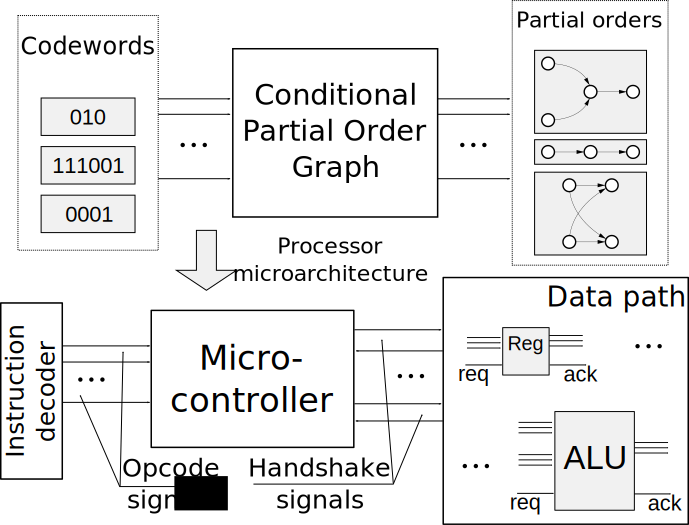
\includegraphics[width=0.6\columnwidth]{fig/control}\vspace{-1mm}

\par\end{centering}

\caption{CPOGs and processor microcontrol\label{fig:Dynamically-reconfigurable-controller}}
\vspace{-3mm}
\end{figure}


Synthesis of instruction sets is a particularly active research area.
There are methods for automated ISA synthesis for a target platform
(according to available system resources and data-path components)
and for given software requirements (e.g. aimed to ease compilation
or reduce program length). These methods eventually produce a structured
set of instructions satisfying certain properties (orthogonality,
completeness, regularity, etc.); instructions are grouped into classes
and each class is allocated a certain opcode interval within the total
code space~\cite{2003_nohl_dac}. At this point automation is typically
stopped or becomes trivial: the instructions are given arbitrary codes
within the allocated intervals. This limits performance due to instruction
decoder circuitry overheads. The problem is usually approached by
ad-hoc heuristics or application-specific optimisation techniques
(see, for example,~\cite{2002_lee_iccad}).

In this paper we try to solve the general problem of optimal encoding
of a given set of instructions with the aid of the Conditional Partial
Order Graph (CPOG) model introduced recently~\cite{2009_mokhov_phd}\cite{2010_mokhov_ieee}.
The key features of the model are: ability to describe systems in
a compact functional form, and structural synthesis methods which
significantly improve performance of the whole design flow. These
features make the model very efficient for representation and management
of processor instruction sets in hardware and EDA software. A CPOG
is a superposition of a set of partial orders which can be extracted
from it by providing the corresponding codewords, see Figure~\ref{fig:Dynamically-reconfigurable-controller}
(top). It can be regarded as a custom associative memory for storing
cause and effect relations within a predefined set of events.

There are different kinds of systems which can be described with the
model. For example, a processor microcontroller executes partial orders
(or \textbf{instructions}) of primitive computational steps (or \textbf{microinstructions})
defined on a set of data path operational units, see Figure~\ref{fig:Dynamically-reconfigurable-controller}
(bottom). The order is determined by an \textbf{instruction}\textbf{\emph{
}}\textbf{code} --- a combination of logical conditions presented
to the controller by the environment~\cite{1994_de_micheli_book}.
To this end, the microcontroller can be seen as an entity which communicates
with two parts of the environment: one part is the source of condition
signals (an instruction decoder) and the other part is a set of controlled
objects with request-acknowledgement interface (data path operational
units which execute the microinstructions).

There are many criteria which determine the choice of a particular
processor architecture and influence design of an instruction set:
functionality, operation modes, resources, etc. In Section~\ref{sec-processor}
we study an example of an instruction set (a subset of \emph{MSP430}
processor~\cite{mspmanual}) implemented on a minimalistic hardware
platform. However, the main focus of this paper is optimal encoding
of processor instruction sets in the general architecture-independent
context. See~\cite{2011_mokhov_tr} for investigation of the architecture-level
reasoning using the CPOG model.

Main contributions of this paper are: firstly, it formulates several
instruction set encoding problems in terms of the CPOG model; secondly,
it presents the SAT characterisation of the problems leading to their
efficient automated solution; thirdly, it demonstrates application
of the CPOG methodology at different stages of a processor design
flow --- from architectural-level specification, design and behavioural
description of an instruction set to its encoding and synthesis of
the physical implementation of the microcontroller. The paper is organised
as follows. Section~\ref{sec:CPOG-model-essentials} briefly introduces
the CPOG model providing a ground for formulating a set of problems
of optimal instruction set encoding in Section~\ref{sec:Optimal-encoding-problem}.
A method for automated translation of the problems into SAT instances
is explained in Section~\ref{sec:SAT-formulation}. It is followed
by a processor design example in Section~\ref{sec-processor} and
conclusions.

\section{Machine-assisted formalisation of parametrised graphs}


Since parametrised graphs are likely to be applied in a safety-critical toolchain, it is imperative to attain a degree of confidence in its properties. Equally important is to convince prospective users that the techniques is sound and lives up to its promises. To fullfil this goal, it was decided to construct in a strict and controlled manner a complete formalisation of the PG formalism. The Agda system \cite{agda} was chosen for its expressive notation language and extensive support for machine-checked formal inference. Agda has enjoyed a notable success as the basis for the formalisation (case studies, success stories)

Says that Agda is LCF, what is LCF. What are the altrenatives: Isaballe/HOL, HOL-Light, ACL2, Coq, PVS, Nqthm. What the have achieved (the colouring problem, pentium div, ...)

compare to Maude (2 lines)

a small agda example: list 

explain why an alegbraic specification is better suited than a model-based (VDM, Z, B) or process based (CSP, CCS).


The new Parametrised Graphs  introducing the following features:
\begin{itemize}
\item{it lifts the assumption of graph acyclicity, allowing general graphs instead of partial orders;}
\item{it adds algebraic operations for combining existing specifications, thus achieving compositionality;}
\item{it axiomatically defines the equivalence relation on specifications, allowing for equivalence preserving transformations.}
\end{itemize}


